\documentclass[extra]{gji}
%~ \documentclass[extra, referee]{gji}

\usepackage[utf8]{inputenc}
\usepackage{timet}
\usepackage{amsmath}
\usepackage{graphicx}
\usepackage{todonotes} % to make annotations on margins
%~ \usepackage[disable]{todonotes} % to disable annotations on margins

\usepackage{url}
\usepackage[pdftex,colorlinks=true]{hyperref}
\hypersetup{
    allcolors=blue,
}


\begin{document}

\title[Variable Density Tesseroids]{
    Gravitational field calculation in spherical coordinates using variable 
    densities in depth
}
\author[S.R. Soler, A. Pesce, L. Uieda and M.E. Gimenez]{
    Santiado R. Soler$^{1,2}$, Agustina Pesce$^{1,2}$, Leonardo Uieda$^3$ and
    Mario E. Gimenez$^{1,2}$ \\
    $^1$CONICET, Argentina. e-mail: santiago.r.soler@gmail.com\\
    $^2$Instituto Geofísico Sismológico Volponi, Universidad Nacional de
    San Juan, Argentina\\
    $^3$Department of Geology and Geophysics, SOEST, University of Hawai‘i at
    Manoa, Honolulu, Hawaii, USA
    }


\maketitle

\begin{summary}
We present a new methodology to compute the gravitational fields generated by 
any tesseroid whose density varies continuously in depth, i.e. a forward 
gravity model in spherical coordinates for varying densities on the radial 
direction.
It numerical approximates these gravitational fields through the 
Gauss-Legendre Quadrature along with two discretization algorithms that 
increase its accuracy by subdividing the tesseroid into smaller ones.
The first one is a preexisting adaptive discretization algorithm that reduces 
the errors due to the distance between the tesseroid and the computation 
point.
While the second one  is a new density-based discretization algorithm that 
decreases the errors introduced by the variation of the density function.
The amount of discretizations made by each algorithm is indirectly controlled 
by two predefined scalar values: the distance-size ratio $D$ for the former 
and the delta ratio $\delta$ for the latter.
We have also obtained analytical solutions for a spherical shell with variable 
density and compared them with the results of the numerical model in case of a 
linear and an exponential density function.
These comparisons allowed to obtain default values for the distance-size and 
the delta ratio in order to guarantee the accuracy of the forward model.
The resulting optimal values of $D$ for the gravity potential, the components 
of its gradient and the Marussi tensor components are 1, 2 and 8, 
respectively.
While a $\delta=0.2$ is needed for the computation of the gravitational 
potential and its gradient components and a $\delta=0.01$ must be used for 
the Marussi tensor components.
We have finally tested this new methodology by modelling the Neuqu\'en 
sedimentary basin, located to the east of the Andes between 32$^\circ$S and 
40$^\circ$S latitude, assigning an exponential density variation to it and 
computing all the gravitational fields it generates.
\end{summary}

\begin{keywords}
Numerical modelling, Numerical approximations and analysis, Gravity anomalies 
and Earth structure, Satellite gravity
\end{keywords}


\section{Introduction}

Lithosphere's density variation with depth has been studied for almost a 
century.
On the first years \citet{Athy1930} obtained a decreasing exponential relation 
between both quantities by studying shale samples, while in the following 
decades other density functions have been proposed for different rock types 
\citep[e.g.,][]{Maxant1980, Rao1986, Rao1993, Rao1994}. 
Furthermore, varying densities have been taken into account in forward and 
inversion gravity models, mostly applied to grabens and basins 
\citep{Cordell1973, Rao1986, Cowie1990, Rao1993, Rao1994, Zhang2001, 
Welford2010}.

These forward gravity models have been developed for two or three dimensional 
bodies in cartesian coordinates that properly fit local scales applications. 
Nevertheless, the latest satellite missions have provided us gravity 
measurements with global coverage, which allow geologists and geophysics to 
perform modelling and interpretation on regional scales. This raises the 
importance of building forward models that reproduce the gravity anomalies for 
such scales.

The main issue that should be overcome is to take into account the curvature 
of the Earth, thus the forward model must be defined in spherical coordinates. 
A common way to achieve this is to discretize the Earth in spherical prisms 
known as tesseroids, which are defined by pairs of latitude, longitude and 
radial boundaries (see Figure \ref{fig:tesseroid-uieda}).
The calculation of the gravitational fields generated by an arbitrary 
tesseroid on any external point involves the resolution of volume 
integrals that are generally approximated by numerical computations.
The literature offers two approaches: one involves Taylor series expansion 
\citep{Heck2007, Grombein2013} while the other makes use of Gauss-Legendre 
Quadrature (GLQ)
\citep{Asgharzadeh2007, Wild-Pfeiffer2008, Uieda2016, Uieda2017}.

In order to develop a forward model that computes the gravitational 
field generated by any tesseroid with arbitrary variable density, the 
Taylor series expansion is not well suited, because it would need the 
series expansion terms for each density function.
On the other hand, the GLQ consists in approximating the integral by a 
weighted sum of the effect of point masses located at scaled nodes of the 
Legendre polynomials, where the density variation is summarised into the 
weights.
Thus, this kind of numerical approximation allows to calculate the 
gravitational fields for any density function without any other 
information but the function itself.

\begin{figure}
\centering
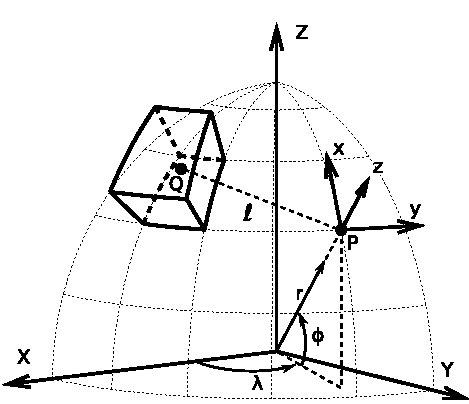
\includegraphics[width=0.9\linewidth]{figures/tesseroid-uieda.pdf}
\caption{
    A spherical prism, also known as  Tesseroid, in a geocentric spherical 
    coordinate system, with a computation point $P$ and its local north 
    oriented Cartesian coordinate system. Picture made by \citet{Uieda2015}.
}
\label{fig:tesseroid-uieda}
\end{figure}

\citet{Uieda2016} developed a forward gravitational model based on 
tesseroids with homogeneous densities using the GLQ approximation 
method.
The main issue of the GLQ is that the approximation becomes less 
accurate when the computation point is closer to the tesseroid or for 
smaller GLQ order \citep{Ku1977}.
Although the model developed by \citet{Uieda2016} uses a second order GLQ, it 
ensures the accuracy through a modified version of the adaptive 
discretization of \citet{Li2011}.
It consist in splitting the tesseroid into smaller ones when a certain 
distance-size ratio is lower than a predefined value ($D$) that controls the 
accuracy of the computation.
\citet{Uieda2016} have also objectively obtained standard values of $D$ 
for gravitational potential, gradients and tensor components comparing 
the numerical model with the fields generated by a spherical shell, 
which constitutes a special case of the volume integrals that has 
analytical solution \citep{LaFehr1991, Mikuska2006, Grombein2013}.
\todo[inline]{citar mas??}

On the other hand, a varying density inside an arbitrary tesseroid 
introduces a new kind of error into the numerical approximation.
This encouraged us to develop a new density-based discretization 
algorithm that divides the tesseroid into smaller ones taking into 
account the variation of the density function.
The number of subdivisions and thus the accuracy of the approximation 
will be controlled by predefined delta ratio $\delta$.

In summary, we present a new forward gravitational model that allows to 
compute the gravitational fields generated by any tesseroid with an 
arbitrary continuous density function on any external point.
It is based on the GLQ approximation whose accuracy is controlled by 
the modified distance-size discretization \citep{Uieda2016} 
and the new density-based discretization algorithms.

In order to ensure the accuracy of the numerical approximation we have 
determined predefined values for the $D$ and $\delta$ parameters by 
comparing the numerical approximation with the analytical solutions for 
a spherical shell with linear and exponential density, which had to be 
derived.

Furthermore, we developed a Python library that implements this forward 
model.
I makes use of some previously existing classes and functions 
from the Python library Fatiando a Terra for geophysical modelling, 
what saved us time and allowed us to focus on the new model.

Furthermore, we have the intention to include it into a future release 
of the Fatiando a Terra library in order to make its distribution and 
maintenance easier.
\todo[inline]{include this?}

In the following sections we will describe how the new algorithm works, its 
theoretical background, obtain default distance-size ratio and delta ratio 
values needed to get a numerical approximation with acceptable accuracy and 
finally show a simple application of the methodology by modelling the Nequen 
basin through a set of tesseroids with exponential density.

%%%%%%%%%%%%%%%%%%%%%%%%%%%%%%%%%%%%%%%%%%%%%%%%%%%%%%%%%%%%%%%%%%%%%%%%%%%%%%

\section{Theory}

The spherical prisms known as tesseroids are mass elements defined in a 
geocentric spherical coordinate system bounded by a pair of parallels, 
a pair of  meridians, and two concentric spherical surfaces.
We define an external computation point $P(r, \phi, \lambda)$ where the 
gravitational fields generated by the tesseroid are going to be calculated 
with respect to the local north oriented Cartesian coordinate system 
located at $P$.
In the special case of homogeneous density, the gravity potential, its 
gradient and the Marussi tensor components can be calculated through 
the integrals obtained by \citet{Grombein2013} \citep[for same notation 
as the one we will use, see][]{Uieda2016}.

In our case, we will assume that the tesseroid has an arbitrary 
variable density in depth, i.e. only depends on the radial spherical 
coordinate.
Thus, the integrals for the gravitational fields are slightly modified:

\begin{equation}
    V(r,\phi,\lambda) = G
    \int\limits_{\lambda_1}^{\lambda_2}
    \int\limits_{\phi_1}^{\phi_2}
    \int\limits_{r_1}^{r_2}
    \frac{\rho(r')}{\ell} \kappa \,  dr' d\phi' d\lambda',
\label{eq:tesseroid-pot}
\end{equation}
\begin{equation}
    g_{\alpha}(r,\phi,\lambda) = G
    \int\limits_{\lambda_1}^{\lambda_2}
    \int\limits_{\phi_1}^{\phi_2}
    \int\limits_{r_1}^{r_2}
    \rho(r') \frac{\Delta_\alpha}{\ell^3}
    \kappa \, dr' d\phi' d\lambda',
\label{eq:tesseroid-grav}
\end{equation}
\begin{equation}
    g_{\alpha\beta}(r,\phi,\lambda) = G
    \int\limits_{\lambda_1}^{\lambda_2}
    \int\limits_{\phi_1}^{\phi_2}
    \int\limits_{r_1}^{r_2}
    \rho(r') I_{\alpha\beta} \, \kappa \, dr' d\phi' d\lambda' ,
    \label{eq:tesseroid-tensor}
\end{equation}

\noindent where

\begin{equation}
    I_{\alpha\beta} =
    \left(
        \frac{3\Delta_{\alpha} \Delta_{\beta}}{\ell^5} -
        \frac{\delta_{\alpha\beta}}{\ell^3}
    \right) ,
    \label{eq:tesseroid-tensor-kernel}
\end{equation}

\noindent $\alpha, \beta \in \{x, y, z\}$, $\rho(r')$ is the density 
function that depends on the radial coordinate, $\delta_{\alpha\beta}$ 
is Kronecker's delta, $G = 6.674\times10^{-11}\, 
\text{m$^3$kg$^{-1}$s$^{-1}$}$ is the gravitational constant and

\begin{equation}
    \Delta_x = r'[\cos\phi\sin\phi' - \sin\phi\cos\phi'
               \cos(\lambda' - \lambda)],
\end{equation}
\begin{equation}
    \Delta_y = r' \cos \phi' \sin(\lambda' - \lambda),
\end{equation}
\begin{equation}
    \Delta_z = r' \cos \psi - r,
\end{equation}
\begin{equation}
    \kappa = {r'}^2 \cos \phi',
\end{equation}
\begin{equation}
    \ell = \sqrt{{r'}^2 + r^2 - 2 r r' \cos \psi},
\label{eq:ell}
\end{equation}
\begin{equation}
    \cos\psi = \sin\phi\sin\phi' + \cos\phi\cos\phi'
                 \cos(\lambda' - \lambda).
\label{eq:cospsi}
\end{equation}

According to \citet[p.~390]{Hildebrand1987}, we can approximate each 
integral on equations \ref{eq:tesseroid-pot}, \ref{eq:tesseroid-grav} 
and \ref{eq:tesseroid-tensor} by applying a $N$th order GLQ, i.e. as 
a weighted sum of the integration kernel evaluated on the roots of the 
$N$th Legendre polynomial.
In the variable density tesseroid case the GLQ is applied in a similar 
way as \citet{Asgharzadeh2007} and \citet{Uieda2016} do, but in this 
scenario the density function must be also evaluated on the quadrature 
nodes:

\iftwocol{
\begin{equation}
    \begin{split}
        \iiint\limits_\Omega \rho(r') g(r', \phi', \lambda') 
        d\Omega \approx& \\
        A 
        \sum\limits_{i=1}^{N^r}
        \sum\limits_{j=1}^{N^\phi}
        \sum\limits_{k=1}^{N^\lambda}
        & W_i^r W_j^\phi W_k^\lambda \rho(r_i) g(r_i, \phi_j, \lambda_k),
    \end{split}
\label{eq:glq-var-dens}
\end{equation}
}{
\begin{equation}
    \iiint\limits_\Omega \rho(r') g(r', \phi', \lambda') d\Omega \approx
    A 
    \sum\limits_{i=1}^{N^r}
    \sum\limits_{j=1}^{N^\phi}
    \sum\limits_{k=1}^{N^\lambda}
    W_i^r W_j^\phi W_k^\lambda \rho(r_i) g(r_i, \phi_j, \lambda_k),
\label{eq:glq-var-dens}
\end{equation}
}

\noindent where

\begin{equation}
    A = 
    \frac{(\lambda_2 - \lambda_1)(\phi_2 - \phi_1)(r_2 - r_1)}{8},
\end{equation}

\noindent $(r_i, \phi_j, \lambda_k)$ are the GLQ nodes and $W_i^r$ are 
the quadrature weights \citep[see their definitions 
on][]{Hildebrand1987}.

From equation \ref{eq:glq-var-dens} we can observe that the GLQ approximates 
the gravitational fields of a tesseroid as the ones generated by $N_\lambda 
N_\phi N_r$ point masses located at the nodes of the Legendre polynomials, in 
the same way as the GLQ works in the homogeneous density case, where $N_i$ ($i 
\in \{ \lambda, \phi, r \}$) are the orders of the quadrature for each 
integration.
Nevertheless, in this new variable density scenario, the information of 
the density function is summarised into the weights by taking into 
account only the values it assumes on those nodes.
Although this may sound discouraging, we intent to prove otherwise and 
show that this method, along with well suited discretization 
algorithms, approximates the gravitational fields with good accuracy.
\todo[inline]{no se si poner esta ultima oracion}

%%%%%%%%%%%%%%%%%%%%%%%%%%%%%%%%%%%%%%%%%%%%%%%%%%%%%%%%%%%%%%%%%%%%%%%%%%%%%%

\section{Methodology}

In a general way, the numerical error of the GLQ is controlled by the 
order of the quadrature: a higher GLQ order produces a more accurate 
approximation \citep{Hildebrand1987}.
This can also be understood in terms of the tesseroid problem: a higher 
quadrature order increases the number of point masses used to compute 
the gravitational fields and thus lowers the numerical error.

This reasoning could lead to a naive methodology in order to ensure 
accurate gravitational field computations: find the order of the 
quadrature that produces an acceptable numerical error.
Nevertheless, this simple proposal has a few problems: (a) it won't be 
efficient \citep{Li2011, Uieda2016} and (b) it couldn't be applied to 
the general case, i.e. the needed quadrature order probably won't be 
the same for every tesseroid, computation point or density function.

That's why we will keep the GLQ order fixed and make use of 
discretization algorithms.
Instead of uniformly increase the number of point masses that 
approximates a certain tesseroid, the discretization algorithms are 
intended to efficiently subdivide the tesseroid into smaller ones and 
apply the GLQ to each one of them.
These algorithms generally involve a discretization inequation that 
controls if the tesseroid should be subdivided or not, and a certain 
predefined parameter that works as a threshold for the discretization 
inequation.

On the variable density tesseroid problem we found two main error 
sources in the GLQ that should be addressed: (a) the distance between 
the tesseroid and the computation point, and (b) 
the variation of the density function.
The former one is also present in the homogeneous density tesseroid 
models, such as the one developed by \citet{Uieda2016}, and could be 
solved by applying a modified version of the adaptive discretization 
algorithm proposed by \citet{Li2011}.
Although for the latter we need to introduce a new density-based 
discretization algorithm that subdivides the tesseroid taking into 
account the variation of its density function.


\subsection{Modified Adaptive Discretization Algorithm}

Studying the homogeneous density tesseroid problem, \citet{Ku1977} 
noticed that keeping the GLQ orders fixed, the approximation 
becomes less accurate when the computation point is closer to the 
tesseroid, making the point masses effect more noticeable than the 
tesseroid we want to approximate.
One way to prevent this could be increasing the GLQ order in case that 
the computation point is near the tesseroid.
This would uniformly increase the number of point masses inside the 
tesseroid volume.

Instead of doing this, \citet{Li2011} proposed an adaptive 
discretization algorithm which essentially consists in dividing the 
tesseroid based on a ratio between the distance to the computation 
point and its dimensions.
This algorithm produces a more efficient computation because the 
increase of point masses is produced where are more needed.

\citet{Uieda2016} proposed a modified version of this algorithm, whose
modifications can be summed up in:
(1) a faster calculation of the distance from the computation point to 
the tesseroid and 
(2) the application of a stack based algorithm that speeds up the 
computation and gives more control over the recursion step.
More specifically, \citet{Uieda2016} redefined the dimensions of an 
arbitrary tesseroid: $L_\lambda$, $L_\phi$ and $L_r$. The former ones 
are the arc-distances measured along its top surface while $L_r$ is the 
difference between the radii of the top and bottom surfaces.

While keeping the GLQ fixed on second orders, the adaptive 
discretization algorithm starts by checking that the following 
inequality is satisfied:

\begin{equation}
    \frac{d}{L_i} \geq D,
\label{eq:distance-size-ratio}
\end{equation}

\noindent where $i \in \{\lambda, \phi, r\}$, $d$ is the distance 
between the geometric centre of the tesseroid and the computation 
point, and $D$ is a predefined value called distance-size ratio.
If the inequality \ref{eq:distance-size-ratio} is not held for at least 
one spherical coordinate, then the tesseroid must be divided by half in 
that direction.
On the contrary, if the inequality is satisfied for every spherical 
coordinate, the algorithm computes the desired gravitational field using the 
GLQ approximation.
A complete description of the modified adaptive discretization 
algorithm can be found in \citet{Uieda2016}.

In summary, the distance-size ratio $D$ determines indirectly how many 
times the tesseroids will be divided, and therefore efficiently 
regulates both the accuracy of the algorithm and its computation time.
Moreover, it limits the computation time by stopping the division of 
the tesseroids when their dimensions are lower than a certain value 
(1mm), assuming that such small tesseroids do not modifies 
significantly the desired gravitational field.

On the other hand, the value assigned to the distance-size ratio $D$ 
cannot be easily related to the error of the approximation, thus the 
choice of the value of $D$ to get an acceptable accuracy must be 
empirically determined beforehand.
In order to overcome this, \citet{Uieda2016} compared the numerical 
computation with the analytical solution for a spherical shell with 
homogeneous density.


\subsection{Density-based Discretization Algorithm}

Variations in the density function of an arbitrary tesseroid introduce 
a new type of error into the numerical approximation: only a few point 
masses would not reproduce the effect of the density variations.
The modified version of the adaptive discretization algorithm may help 
in reducing this kind of error, but as it only takes into account the 
dimensions of the tesseroid and the distance to the computation point, 
it's not well suited to fully perform this task.

In order to overcome this, we developed a complementary discretization 
algorithm that takes into account the variation of the density inside 
the tesseroid.
Basically, it subdivides any tesseroid on the radial direction on the 
depth at which the \emph{maximum density variation} takes place, only 
if a certain discretization inequation holds.

\begin{figure*}
\centering
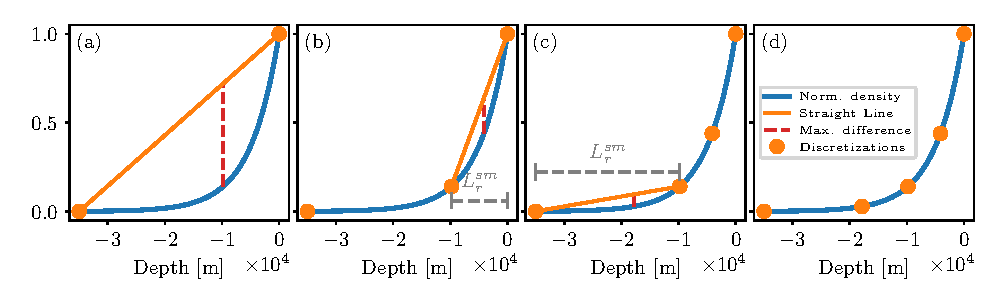
\includegraphics[width=\linewidth]
    {figures/density-based-discretization-algorithm.pdf}
\caption{
    Example intended to show how the density-based algorithm works.}
\label{fig:density-discretization-algorithm}
\end{figure*}

In a general way, the algorithm can be summarised in the following steps:

\begin{enumerate}
\renewcommand{\theenumi}{(\arabic{enumi})}
    \item Normalise the density function to the [0, 1] interval,
    \item Compute the absolute difference between the normalised 
          density and a linear function that assumes the same values on the 
          top and bottom radii that this normalised density.
    \item If product of the maximum of the absolute difference and a 
          tesseroid size ratio is greater that a predefined delta ratio 
          ($\delta$), then the tesseroid will be subdivided on the 
          radius at which this maximum takes place. Otherwise, the 
          tesseroid won't be split.
    \item If it's discretized, then apply items (2), (3) and (4) for 
          every subdividing tesseroid.
\end{enumerate}

Lets assume an arbitrary \emph{original} tesseroid with boundary radii 
$R_1$ and $R_2$ and a density function $\rho(r')$, whose radial 
dimension is $L_r = R_2 - R_1$.

First we need to normalise the density function such as its minimum and 
maximum will be 0 and 1, respectively.
We call this normalised density $\rho_n(r')$ and we calculate it as 
follows:

\begin{equation}
    \rho_n(r') =
    \frac{\rho(r') - \rho_\text{min}}{\rho_\text{max} - \rho_\text{min}},
\end{equation}
\noindent where
\begin{equation}
    \rho_\text{min} = \text{min}\{ \rho(r') \}, \quad
    \rho_\text{max} = \text{max}\{ \rho(r') \} \quad
    \forall \, r' \in [R_1, R_2].
\end{equation}

\noindent Because the algorithm will be iteratively applied for every 
subdividing tesseroid, we'd like to note that this normalised density 
function will be the same for every subdividing tesseroid.
In case that the density function is constant, both the maximum and 
minimum densities are equal and the normalised function could not 
be defined, so the density-based discretization algorithm won't be 
applied.

Secondly, we must define a linear function $\rho_l(r')$ that assumes 
the same values as the normalised density $\rho_n(r')$ on the boundary 
radii $R_1$ and $R_2$:

\begin{equation}
    \rho_l(r') =
    \frac{ \rho_n(R_2) - \rho_n(R_1) }{ R_2 - R_1 } (r' - R_1) + \rho_n(R_1),
    \label{eq:density-reference-line}
\end{equation}

\noindent and compute the absolute difference between this linear 
function and the normalised density:

\begin{equation}
    \Delta \rho (r') = | \rho_n(r') - \rho_l(r') |.
    \label{eq:density-abs-diff}
\end{equation}

Finally, if the following inequation holds, the tesseroid will be divided on 
the radius $R_\text{max}$ at which the maximum absolute difference takes 
place:

\begin{equation}
    \text{max}\{ \Delta \rho(r') \} \frac{L_r^\text{sm}}{L_r} > \delta,
    \label{eq:delta-density}
\end{equation}

\noindent where the delta ratio $\delta$ is a predefined constant value and 
$L_r^\text{sm}/L_r$ is defined as the tesseroid size ratio, while 
$L_r^\text{sm}$ and $L_r$ are the radial dimensions of the tesseroid that is 
currently analysed and of the \emph{original} one, respectively.
On the first iteration, the former tesseroid corresponds to the 
\emph{original} one, so $L_r^\text{sm}/L_r$ is equal to one, but for 
future iterations this radial dimension will be computed as the 
difference of the top and bottom radii of the subdividing tesseroid, making 
$L_r^\text{sm}/L_r$ lower than one.
The tesseroid size ratio is intended to reduce the number of unneeded 
discretizations and focus on the ones that will significantly reduce the 
numerical error:
a big subdividing tesseroid with small maximum absolute difference would 
cause more relative numerical error than a small subdividing tesseroid with 
higher maximum absolute difference.

Once the \emph{original} tesseroid is discretized, we proceed to 
subsequently apply the same algorithm on every subdividing tesseroid.
We will start from equation \ref{eq:density-reference-line} defining a 
new linear function $\rho_l(r')$, an absolute difference with equation 
\ref{eq:density-abs-diff} and evaluate the discretization inequation 
\ref{eq:delta-density}, taking into account that now $R_1$ and $R_2$ 
are the radial boundaries of this smaller tesseroid.
If the inequation holds, the current tesseroid is discretized and the 
algorithm is subsequently applied to the resulting subdividing tesseroids.

If on the contrary the inequation \ref{eq:delta-density} is not held, 
then the tesseroid will not be discretized.
The same happens if the tesseroid radial dimension is bellow the 
threshold of 1mm.
On the first case due to the fact that no more discretizations are 
needed, and on the second one because smaller tesseroids will not 
introduce meaningful increases in the accuracy of the computation.
This two conditions guarantee that the algorithm is finite.
Once any of them is met and no more discretizations are carried out, 
every subdividing tesseroid is subjected to the modified adaptive 
discretization algorithm and then a second order GLQ will be applied in 
order to compute the gravitational field generated by it.

On Figure \ref{fig:density-discretization-algorithm}(a) we propose an 
arbitrary normalised density function as an example of how this 
algorithm works.
We plotted its corresponding linear function $\rho_l(r')$ and a 
dashed line that represents the maximum absolute difference.
We will assume that the discretization inequation 
\ref{eq:delta-density} holds in this case, so we must divide the 
tesseroid at the depth at which the maximum difference occurs.
The dots on Figure \ref{fig:density-discretization-algorithm} 
represent the discretization points, i.e. the radial boundaries of the 
subdividing tesseroids produced by the algorithm.

On Figure \ref{fig:density-discretization-algorithm}(b) we apply the 
algorithm on the shallower subdividing tesseroid.
In the same way, we plot the linear function and compute the maximum 
absolute difference $\Delta \rho (r')$.
In this case, the tesseroid size-ratio $L_r^\text{sm}/L_r$ is lower 
than one and will be taken into account in the discretization 
inequation, which will be assumed to hold also in this case, leading to 
the division of this tesseroid.

On Figure \ref{fig:density-discretization-algorithm}(c) we perform the 
same analysis on the deeper subdividing tesseroid, and assuming that the 
inequality holds in this case we also subdivide it.

Finally, if we suppose that the value of $\delta$ used in this example 
does not produce further discretizations, the resulting subdividing 
tesseroids can be seen on Figure 
\ref{fig:density-discretization-algorithm}(d).

It's easy to see that the delta ratio indirectly controls how many 
times the tesseroids will be subdivided based on the variation of the 
density function.
Therefore it determines the accuracy involving the numerical error that 
the density variation introduces and also the computation time: a lower 
value of $\delta$ will produce more discretizations leading to an 
increase in the accuracy of the approximation but also in the 
computation time.
This raises the need to determine a maximum value of $\delta$ that 
ensures an acceptable accuracy while minimising the computation time.


\subsection{Algorithm summary}

When computing any gravitational field generated by an arbitrary tesseroid on 
a specific computation point, we present the following methodology:

\begin{enumerate}
    \renewcommand{\theenumi}{(\arabic{enumi})}
    \item Apply the density-based discretization algorithm in case of 
          variable density producing subdivisions of the original tesseroid,
    \item Apply the modified adaptive discretization algorithm for 
          each subdivision, generating a set of smaller tesseroids,
    \item Compute the desired gravitational field for every small tesseroid 
          through the GLQ approximation with fixed quadrature orders
          (equation \ref{eq:glq-var-dens}).
\end{enumerate}

In most practical cases, the forward model will consist in a set of 
tesseroids whose gravitational effect will be computed on a set of 
computation points.
These steps can be applied on every tesseroid and for each computation point,
adding the contribution of each tesseroid to the resulting 
gravitational field.


%%%%%%%%%%%%%%%%%%%%%%%%%%%%%%%%%%%%%%%%%%%%%%%%%%%%%%%%%%%%%%%%%%%%%%%%%%%%%

\section{Determination of distance-size and delta ratios}

The discretization algorithms described on the previous section are 
introduced to improve the accuracy of the numerical approximation of 
the gravitational fields.
They involve two predefined ratios that determine how many 
times each tesseroid will be discretized and thus indirectly control 
the numerical error of the approximation.
The modified version of the adaptive discretization algorithm involves  
the distance-size ratio $D$, while the density-based discretization 
algorithm makes use of the delta ratio $\delta$.
These algorithms need predefined default values for $D$ and $\delta$ 
in order to ensure both acceptable numerical accuracy and computation 
effectiveness.

On the homogeneous density tesseroids case, \citet{Uieda2016} compared 
their numerical model with the analytical solution of a spherical 
shell in order to obtain default values for the distance-size ratio 
$D$.
We could follow this idea, but for our needs the spherical shell must 
have the same density function as the numerical model.
In contrast with the homogeneous density case, the analytical solutions 
for a variable density spherical shell are not present in the 
literature, so they must be obtained.

We will then perform these comparisons between the analytical solutions 
and the numerical model for specific density functions: a linear and an 
exponential one.
From these results we will finally obtain default values for $D$ 
and $\delta$ that ensure a numerical error lower than 0.1\%.


\subsection{Analytical Solutions for Spherical Shell}

The integrals that define the gravity fields in equations 
\ref{eq:tesseroid-pot}-\ref{eq:tesseroid-tensor} have almost trivial 
analytical solutions in case of a spherical shell with homogeneous 
density \citep{Mikuska2006,Grombein2013}.
But for a variable density spherical shell the problem haven't been 
addressed in the literature yet.

Lets consider a spherical shell with inner and outer radii $R_1$ and 
$R_2$, respectively, whose density depends on the radial spherical 
coordinate (Figure \ref{fig:spherical-shell}).
The gravity potential generated by the shell on an arbitrary external 
point $Q(0,0,r)$, located along the $z$ axe at a distance $r$ from the 
origin, can be written as follows:

\begin{figure}
\centering
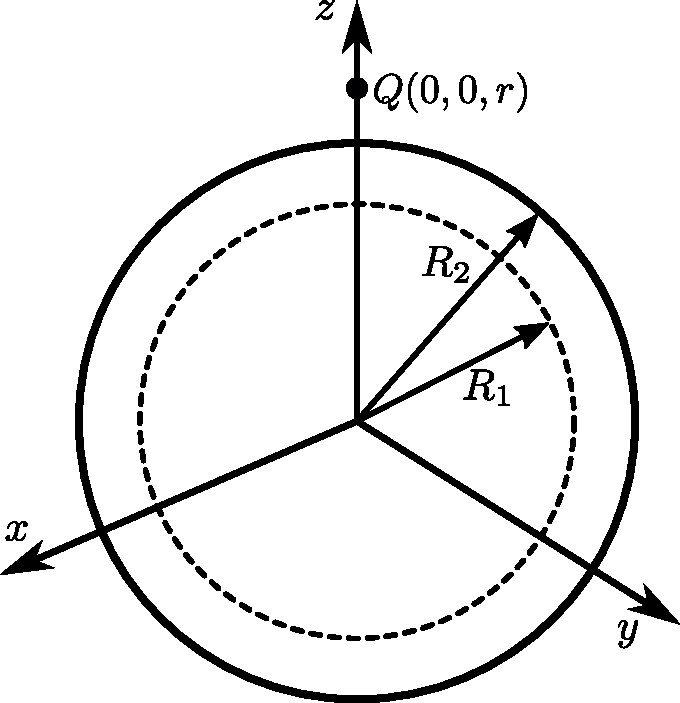
\includegraphics[width=0.7\linewidth]{figures/spherical-shell.pdf}
\caption{
    Spherical shell with inner and outer radii $R_1$ and $R_2$, respectively.
    The computation point $Q$ is located on the $z$ axe at a distance $r$ from
    the centre of the shell.
    For our purposes we will assume that $Q$ is outside the outer radii,
    i.e. $r > R_2$.
    }
\label{fig:spherical-shell}
\end{figure}

\begin{equation}
    V_\text{sh}(r) = G 
    \int\limits_0^{2\pi}
    \int\limits_{-\frac{\pi}{2}}^\frac{\pi}{2}
    \int\limits_{R_1}^{R_2}
    \frac{\rho(r')}{\ell} {r'}^2 \cos\phi' \, 
    dr' d\phi' d\lambda',
\end{equation}

\noindent where $\ell$ is defined in equation \ref{eq:ell}. The computation 
point $Q$ is located at latitude $\phi=90^\circ$, so $\ell$ and $\cos\psi$ 
(defined on equations \ref{eq:ell} and \ref{eq:cospsi}) get simplified:

\begin{equation}
    \cos\psi = \sin\phi', \quad
    \ell = \sqrt{r'^2 + r^2 - 2 r r' \sin\phi'}.
\end{equation}

Due to the rotational symmetry along the $z$ axe, the integration in 
$\lambda'$ is straightforward:

\begin{equation}
    V_\text{sh}(r) = 2\pi G 
    \int\limits_{-\frac{\pi}{2}}^\frac{\pi}{2}
    \int\limits_{R_1}^{R_2}
    \frac{\rho(r') {r'}^2 \cos\phi'}{\sqrt{r'^2 + r^2 - 2 r r' \sin\phi'}}
    \, dr' d\phi',
\end{equation}

\noindent while the integration in $\phi'$ can be performed 
independently of the density function.
Making use of SymPy \citep{sympy2017}, a Python library for symbolic 
mathematics, we obtained the following expression for the potential:

\iftwocol{
\begin{equation}
    \begin{split}
        V_\text{sh}(r) = 2\pi G
        \int\limits_{R_1}^{R_2}
        \Big[ & \sqrt{r^2 + r'^2 + 2rr'} - \\
        & \sqrt{r^2 + r'^2 - 2rr'}
        \Big] \frac{r'\rho(r')}{r} \, dr'.
    \end{split}
\label{eq:shell-pot-sqrts}
\end{equation}
}{
\begin{equation}
    V_\text{sh}(r) = 2\pi G
    \int\limits_{R_1}^{R_2}
    \Big[ \sqrt{r^2 + r'^2 + 2rr'}  -
    \sqrt{r^2 + r'^2 - 2rr'} 
    \Big] \frac{r'\rho(r')}{r} \, dr'.
\label{eq:shell-pot-sqrts}
\end{equation}
}

For our purposes we can assume that the computation point $Q$ is 
farther from the origin than the outer radius, i.e. $r>R_2$. 
And taking into account that $r'$ is always lower than $R_2$, we can 
simplify the square roots in equation \ref{eq:shell-pot-sqrts}:

\begin{equation}
    \sqrt{r^2 + r'^2 + 2rr'} = |r + r'| = r + r',
\end{equation}
\begin{equation}
    \sqrt{r^2 + r'^2 - 2rr'} = |r - r'| = r - r',
\end{equation}

\noindent what leads to the following expression of the potential:

\begin{equation}
    V_\text{sh}(r) = \frac{4\pi G}{r}
    \int\limits_{R_1}^{R_2} {r'}^2 \rho(r') \, dr'.
\label{eq:shell-pot}
\end{equation}

The equation \ref{eq:shell-pot} allows to easily obtain the exact 
gravity potential generated by a spherical shell with a variable 
density in depth on any outside point located on the $z$ axe.
Due to the rotational symmetry along any axe that passes through the 
centre of the shell, the expression in equation \ref{eq:shell-pot} 
reproduces the gravity potential field on any outside point at distance 
$r$ from its centre.

The gradient and the Marussi tensor derived from potentials that 
depends solely on $r$ have only a few non zero components: the vertical 
component of the gradient ($g_z$) and the diagonal components of the 
tensor ($g_{xx}$, $g_{yy}$, $g_{zz}$).
They can be easily obtained as \citet{Grombein2013} does, even for any 
arbitrary density function $\rho(r')$:

\begin{equation}
    g_z = \frac{V_\text{sh}(r)}{r},
\end{equation}
\begin{equation}
    g_{xx} = g_{yy} = -\frac{V_\text{sh}(r)}{r^2}, \quad
    g_{zz} = \frac{2V_\text{sh}(r)}{r^2}.
\end{equation}


\subsection{Linear Density}

Lets perform a comparison between our numerical model and the 
analytical solution for a spherical shell with a linear density 
function like the following one:

\begin{equation}
    \rho(r') = ar' + b.
\end{equation}

First, by solving the integral on equation \ref{eq:shell-pot}, we obtained the 
gravitational potential generated by a spherical shell with this density on 
any external point at distance $r$ from its centre:

\begin{equation}
    V_\text{sh}^\text{lin}(r) = \pi G \left[ 
    a \frac{R_2^4 - R_1^4}{r} +
    b \,\frac{4}{3} \frac{R_2^3 - R_1^3}{r} \right].
    \label{eq:shell-pot-linear}
\end{equation}

\noindent The first term on this equation reproduces the potential generated 
by a spherical shell with variable density $\rho(r') = ar'$, while the second 
one constitutes the potential generated by a spherical shell with homogeneous 
density $\rho = b$ \citep{Mikuska2006,Grombein2013}.

Secondly we can analyse how the density-based discretization algorithm 
works in case of a linear density function.
Because the absolute difference defined on equation 
\ref{eq:density-abs-diff} will always be zero, the discretization 
inequation \ref{eq:delta-density} will never be satisfied.
Therefore, independently of the linear function proposed, the 
density-based algorithm will never be applied, leaving the modified 
adaptive discretization algorithm as the only mechanism to control the 
accuracy of the numerical approximation.
That's why, for linear density scenarios, we only need to determine 
the minimum value of $D$ needed in order to guarantee an acceptable 
accuracy while ignoring the value of $\delta$.

In order to compare the numerical model with the analytical solution we 
must build a spherical shell made of tesseroids.
We propose a mesh of $30^\circ \times 30^\circ$ tesseroids whose outer and 
inner radii are the same ones as the spherical shell in order to compute 
the gravitational potential, the vertical component of the gradient 
($g_z$) and the diagonal components of the Marussi tensor ($g_{xx}$, 
$g_{yy}$, $g_{zz}$) on four different grids: (1) a grid located at the 
pole, (2) another one on the Equator, (3) one located at satellite 
height and (4) a big grid of $30^\circ \times 30^\circ$.
More information about this grids can be found on Table 
\ref{tab:grids}.

We will compute these gravitational fields on every point of the four 
grids for different values of $D$, ranging from 0.5 to 10 with a step 
of 0.5.
Then we will calculate the maximum difference between these results and the 
value that the analytical solution assumes at the same height of the 
computation grid.
Because the gravity fields generated by a tesseroid are approximated by 
the effect of point masses, the numerical results may vary between 
computation points at same height but at different latitude or 
longitude.
That's why we will choose for comparison the maximum difference between the 
results on every point of the grid and the analytical solution.

Finally, we will set the acceptable value of $D$ as the minimum value 
at which the corresponding error of the numerical approximation is 
lower than 0.1\%.

\begin{table}
\caption{
    Description of the synthetic grids on which the comparison of the 
    numerical model against the analytical solutions for a spherical 
    shell was done.
    This collection of grids tries to include every possible scenario 
    on which the numerical model can present a different behaviour 
    depending on the size of the grid, its location or its height over 
    the Earth surface. Every grid consists in a set of 10$\times$10 
    points.
}
\label{tab:grids}
\begin{tabular}{lcccc}
    Grid & Size & Lat. extension & Lon. extension & Height \\ \hline
    Pole & $1^\circ \times 1^\circ$ & $89^\circ - 90^\circ$ &
        $0^\circ - 1^\circ$ & 2km \\
    Equator & $1^\circ \times 1^\circ$ & $0^\circ - 1^\circ$ &
        $0^\circ - 1^\circ$ & 2km \\
    Satellite & $1^\circ \times 1^\circ$ & $89^\circ - 90^\circ$ &
        $0^\circ - 1^\circ$ & 260km \\
    Big Grid & $30^\circ \times 30^\circ$ & $60^\circ - 90^\circ$ &
        $0^\circ - 30^\circ$ & 2km \\
\end{tabular}
\end{table}

In order to perform the comparison, we proposed a thin and a thick 
spherical shells with 1km and 35km of thickness, respectively, whose 
outer radii are equal to the mean Earth radius.
On both cases we will suppose that the density assumes a value of 
2670~kg/m$^3$ on the outer surface and 3300~kg/m$^3$ at the inner 
radius:

\begin{equation}
    \rho(r') = ar' + c,
    \label{eq:density-linear}
\end{equation}
\noindent with 
\begin{equation}
    a = -\frac{3300\text{kg/m$^3$} - 2670\text{kg/m$^3$}}{R_2 - R_1},
\end{equation}
\begin{equation}
    c = \frac{3300\text{kg/m$^3$} - 
        2670\text{kg/m$^3$}}{R_2 - R_1} R + 
        2670\text{kg/m$^3$},
\end{equation}

\noindent where $R$ = 6378.137 km is the mean Earth radius.

We have computed the percentage difference between the numerical model 
with its corresponding analytical solution (equation 
\ref{eq:shell-pot-linear}) for the thick and the thin spherical shell 
on each of the four grids described in Table \ref{tab:grids}.
We can see the results for the potential, the vertical component of the 
gradient $g_z$ and the $g_{zz}$ component of the Marussi tensor on 
Figure \ref{fig:D-linear}.
We exclude the results corresponding to the other two diagonal 
components of the tensor because they are similar to the ones obtained 
for the $g_{zz}$, although they can be found on the repository. 
\todo[inline]{chequear}

For the linear density case, we can observe that the calculation of the 
potential and the $g_z$ component of its gradient needs a value of 
$D=1$ and $D=2$, respectively, in order to ensure a numerical error 
bellow the 0.1\% threshold.
On the other hand, the $g_{zz}$ computations show a noticeable 
difference between the thin and the thick shell: the first one needs a 
value of $D$ equal to 8 while the later only a $D$ of 3.5.
We will keep the more conservative result of $D$ equal to 8 in case of 
computing the Marussi tensor components.

\begin{figure*}
\centering
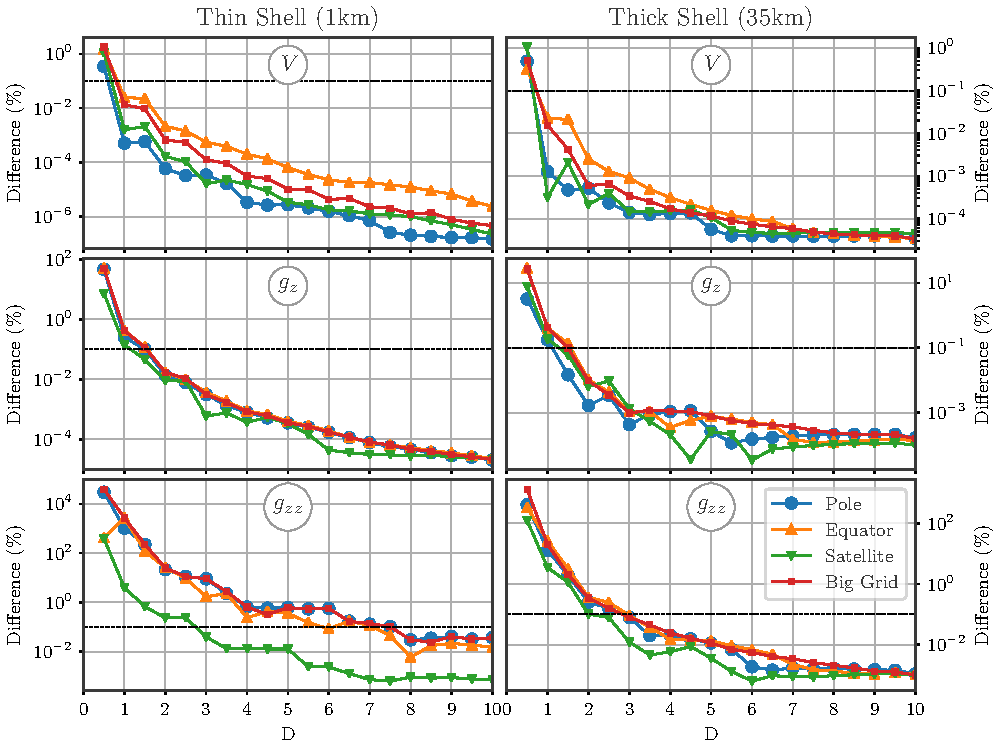
\includegraphics[width=\linewidth]{figures/linear-D.pdf}
\caption{
    Differences between the gravity fields generated by the numerical model 
    and the analytical solution for a thin and a thick spherical shell of 1km 
    and 35km of thickness, respectively.
    Both models have the linear density defined on equation 
    \ref{eq:density-linear}.
    The computations were performed on the four grids described in 
    Table \ref{tab:grids}, for different values of the distance-size 
    ratio $D$.
    Due to the linearity of the density function, the density-based 
    discretization algorithm is not applied.
    If the difference is less than 0.1\%, we consider that the model 
    has achieved an acceptable accuracy for the corresponding value of 
    $D$.
    }
\label{fig:D-linear}
\end{figure*}


\subsection{Exponential Density}

Lets perform a similar comparison between the numerical model and 
the analytical solution but now for a spherical shell with exponential 
density.
On this scenario the problem is more complex due to the fact that the 
density-based discretization will be certainly applied together with 
the modified adaptive discretization algorithm.
This means that both the distance-size ratio $D$ and the delta ratio 
$\delta$ must be simultaneously determined.

\subsubsection{$D$, $\delta$ space exploration}

From every combination of the $D$ and $\delta$ ratios we want to find 
the one that produces a numerical error lower than the 0.1\% threshold 
while keeping an effective computation, i.e. the ($D$, $\delta)$ pair 
that produces the minimum number of discretizations and ensures an 
acceptable numerical precision.
We can propose an heuristic method to perform this task: compute the 
numerical error for every ($D$, $\delta$) points belonging to a grid on 
the $D$, $\delta$ space and choose the pair that combines an 
acceptable numerical error with an efficient computation.

Firstly, lets consider a decreasing exponential density function that 
assumes the values of 2670 kg/m$^3$ and 3300 kg/m$^3$ on the shell's 
outer and inner radii, respectively, that can be defined as follows:

\begin{equation}
    \rho(r') = A e^{-(r' - R)/b} + C,
\label{eq:density-exp}
\end{equation}
\noindent where
\begin{equation}
    A =
    (3300 \text{kg/m}^3 - 2670 \text{kg/m}^3)
    \left( e^{( R_2 - R_1 )/b} - 1 \right)^{-1},
\end{equation}
\begin{equation}
    C =
    2670 \text{kg/m}^3 - A,
\end{equation}

\noindent $R$ is the mean Earth radius and $b$ is a constant 
that determines the variability of the function: a low value of $b$ 
increases the maximum slope of the density function.
The analytical solution of the gravitational potential generated by a 
spherical shell with a density functions as the one in equation 
\ref{eq:density-exp} can be obtained by solving the equation 
\ref{eq:shell-pot} as follows:

\iftwocol{
\begin{equation}
    \begin{split}
        V_\text{sh}^\text{exp}(r) = \frac{4\pi G}{r} 
        Ab 
        \Big[
        & (R_1^2 + 2R_1 b + 2b^2)e^{-\frac{R_1 - \Delta h}{b}} - \\
        & (R_2^2 + 2R_2 b + 2b^2)e^{-\frac{R_2 - \Delta h}{b}}
        \Big] + \\
        & \frac{4 \pi G}{3 r} C (R_2^3 - R_1^3).
    \end{split}
\label{eq:shell-pot-exp}
\end{equation}
}{
\begin{equation}
    V_\text{sh}^\text{exp}(r) = \frac{4\pi G}{r} 
    Ab \, e^\frac{\Delta h}{b}
    \Big[
    (R_1^2 + 2R_1 b + 2b^2)e^{-\frac{R_1}{b}} -
    (R_2^2 + 2R_2 b + 2b^2)e^{-\frac{R_2}{b}}
    \Big] +
    \frac{4 \pi G}{3 r} C (R_2^3 - R_1^3).
\label{eq:shell-pot-exp}
\end{equation}
}

Secondly, we propose a thick spherical shell with a thickness of 35km and 
modelled by a mesh of $30^\circ \times 30^\circ$ tesseroids in order to 
perform the exploration of the numerical error in the $D$, $\delta$ 
space.
We have assigned the density function proposed on equation 
\ref{eq:density-exp} to our spherical shell model with a $b$ value of 
1km, i.e. a highly varying density function.

Finally, we have computed the gravitational potential ($V$), the vertical 
component of its gradient ($g_z$) and the $g_{zz}$ component of the 
Marussi tensor on the big grid (see Table \ref{tab:grids}) by exploring 
different values of $D$ and $\delta$.
These results were used to obtain the percentage difference between 
them and their corresponding analytical solutions.

On Figure \ref{fig:grid-search} we show 
the resulting percentage difference for each gravitational field.
The points inside the dotted lines are the ones that present a 
numerical error lower than the 0.1\% threshold.
Our intention is to choose the one that produces the most efficient computation
and set it as the default values for $D$ and $\delta$.

\begin{figure}
\centering
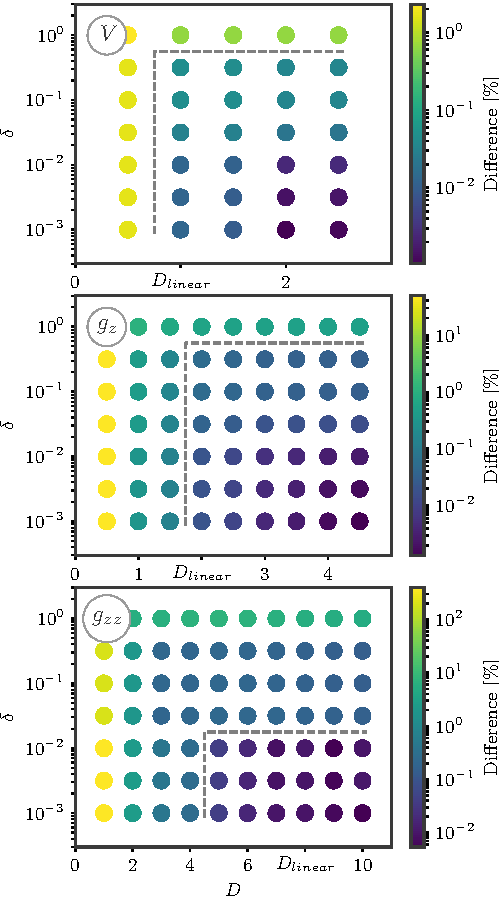
\includegraphics[width=\linewidth]
    {figures/grid-search.pdf}
\caption{
    Numerical error exploration in the $D$, $\delta$ space.
    The percentage difference values were obtained from the comparison 
    between the analytical solution and the numerical approximation of 
    the gravitational fields ($V$, $g_z$ and $g_{zz}$) generated by a 
    spherical shell with an exponential density as the one defined on 
    equation \ref{eq:density-exp}.
    These comparison have been carried out with a spherical shell of 
    35km of thickness, whose density function has a value of $b$ of 1km 
    and the gravitational fields were computed on the big grid 
    (defined in Table \ref{tab:grids}).
    The points inside the dashed line are the ones that present an 
    error lower than 0.1\%.
    }
\label{fig:grid-search}
\end{figure}


\begin{figure}
\centering
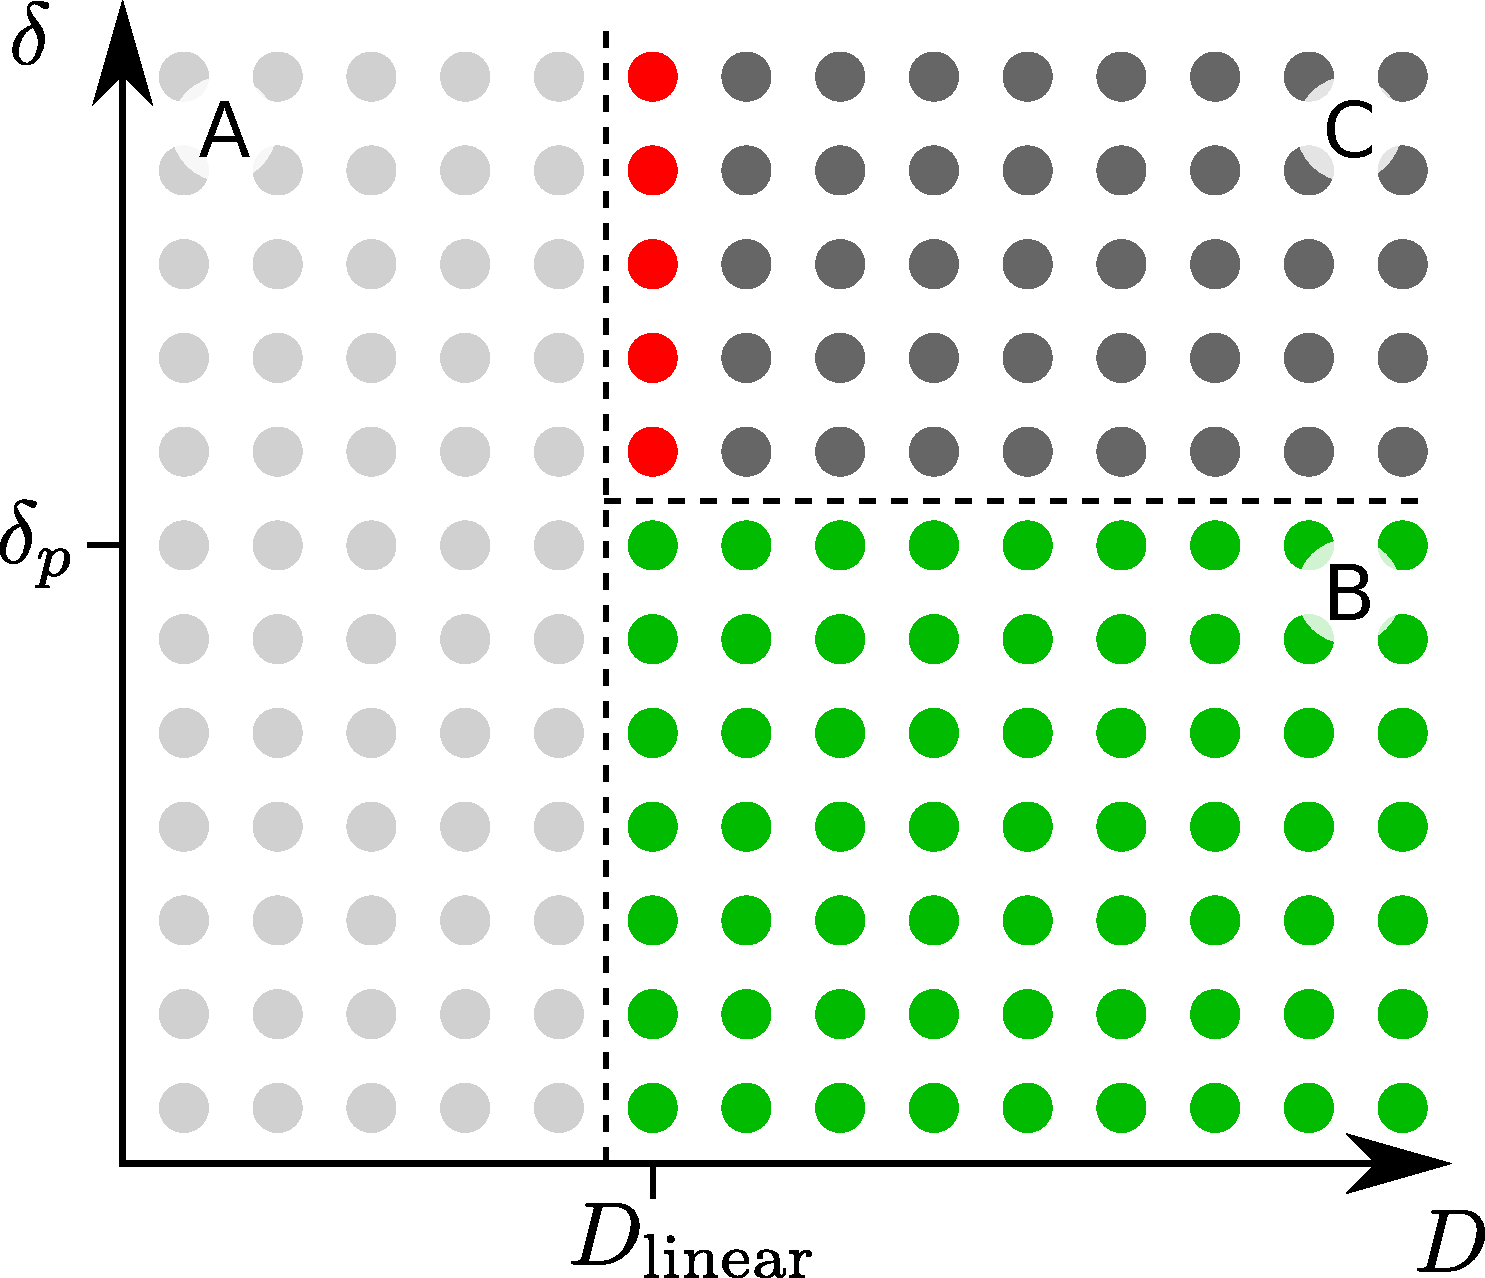
\includegraphics[width=\linewidth]
    {figures/D-delta-grid-search.pdf}
\caption{
    $D$, $\delta$ space divided in three regions (A, B and C) based on 
    the definitions of $D_\text{linear}$ and $\delta_p$ (see text for more 
    information).
    Light grey points are the non-eligible ($D$, $\delta$) pairs 
    belonging to the region A (with $D < D_\text{linear}$).
    Green points have acceptable numerical error (lower than 0.1\%), 
    while the red ones represent those whose error is greater than the 
    threshold.
    Dark grey points represent those from which we don't have a priori 
    information about their numerical error.}
\label{fig:D-delta-grid-search}
\end{figure}

Because the algorithm is thought to work with default $D$ and $\delta$ 
values that ensures these two conditions for every density function, 
the default value for $D$ cannot be lower than the one determined for 
the linear function, which will be called $D_\text{linear}$.
That's why we can only choose the ($D$, $\delta$) points on which
$D \geq D_\text{linear}$.
Taking this fact into account we can divide the $D$, $\delta$ space in 
two subregions: one with $D < D_\text{linear}$ and other with $D \ge 
D_\text{linear}$.
We can ignore points belonging to the former one (region A on Figure 
\ref{fig:D-delta-grid-search}) and focus on the latter (regions B and C on 
Figure \ref{fig:D-delta-grid-search}).

From the $D \ge D_\text{linear}$ subregion we can explore the numerical 
error of points with $D = D_\text{linear}$ and different values of 
$\delta$.
We will call $\delta_p$ to the maximum $\delta$ at which the numerical 
error is lower than the 0.1\% threshold while keeping
$D = D_ \text{linear}$.
Greater $\delta$ values than $\delta_p$ will produce computations with 
high error (red points in Figure \ref{fig:D-delta-grid-search}), while 
lower $\delta$ values than $\delta_p$ will produce more discretizations 
leading to non-efficient computation (green dots under the 
$(D_\text{linear}, \delta_p)$ point on Figure \ref{fig:D-delta-grid-search}).

With the definition of $\delta_p$ in mind we can subdivide the 
subregion in two: one with points with $\delta \le \delta_p$ (region B 
on Figure \ref{fig:D-delta-grid-search}) and other with points with 
$\delta > \delta_p$ (region C on Figure \ref{fig:D-delta-grid-search}).

Every point in the subregion with $\delta \le \delta_p$ (region B on 
Figure \ref{fig:D-delta-grid-search}) will have a numerical error lower 
than the 0.1\% threshold, but they will always produce more 
discretizations than the ($D_\text{linear}$, $\delta_p$) point leading 
to non-efficient computations.
It's worth remembering that a lower $\delta$ or a greter $D$ will 
produce more discretizations, increasing the accuracy but also the 
computation time.

On the other hand, we have no a priori information about the numerical 
error of points with $\delta > \delta_p$ (region C on 
Figure \ref{fig:D-delta-grid-search}).
Nevertheless, the numerical error exploration shown on
Figure \ref{fig:grid-search} doesn't present any 
point in this region with error lower than the threshold.
Even though we are analysing a single case, it proves that no point in 
region C is eligible as default ($D$, $\delta$) pair because it should 
ensure numerical accuracy for every exponential density scenario.

In conclusion, the ($D$, $\delta$) point that minimises the number of 
discretizations while keeping an acceptable numerical error under the 
0.1\% threshold is the one whose ratio $D$ is equal to 
$D_\text{linear}$ and its delta ratio is $\delta_p$.

\subsubsection{Delta ratio determination}

In order to determine a default value of $\delta$ that ensures an 
acceptable accuracy for every exponential density case we have 
performed comparisons between the numerical model and the analytical 
solutions, keeping the distance-size ratio $D$ equal to the values 
obtained for the linear density case while exploring different values of 
$\delta$.

Firstly, we have considered the same spherical shell models we have 
used in the linear density case: a thin one (1km of thickness) and a 
thick one (35km of thickness) composed by $30^\circ \times 30^\circ$ 
tesseroids.
But in this case, we assigned an exponential density function like the 
one shown in equation \ref{eq:density-exp} to each shell, choosing 
a few values of $b$ in order to explore different density 
variations.

Finally, we have computed the gravitational potential ($V$), the 
vertical component of its gradient ($g_z$) and the $g_{zz}$ component of 
the Marussi tensor on the big grid (see Table \ref{tab:grids}) and 
calculated the percentage difference between these numerical results and 
their corresponding analytical solutions.
Our intention is to set the default $\delta$ as the highest value whose 
numerical error is bellow the $0.1\%$ threshold.

On Figure \ref{fig:delta-exponential} we show the density functions 
used on each comparison and the resulting percentage difference for each 
gravitational field.
The first column shows the results for the thin spherical shell, while the 
second one shows the ones corresponding to the thick shell.
From these we can conclude that a $\delta = 0.2$ is needed in order to 
achieve an acceptable numerical error for the computation of the 
potential and the $g_z$ component.
Because the same comparison using the other components of the gradient ($g_x$ 
and $g_y$) could not be carried out, we will extrapolate this result 
setting a default $\delta = 0.2$ for their computation.

On the other hand, the comparison with the $g_{zz}$ component of the 
Tensor shows a difference between the thin and the thick spherical 
shell: the former needs a $\delta = 0.2$, but the latter requires a 
$\delta = 0.01$.
In order to guarantee a good accuracy for every case, we will keep the 
more conservative value of $\delta = 0.01$ for the computation of the 
Marussi tensor components.

\begin{figure*}
\centering
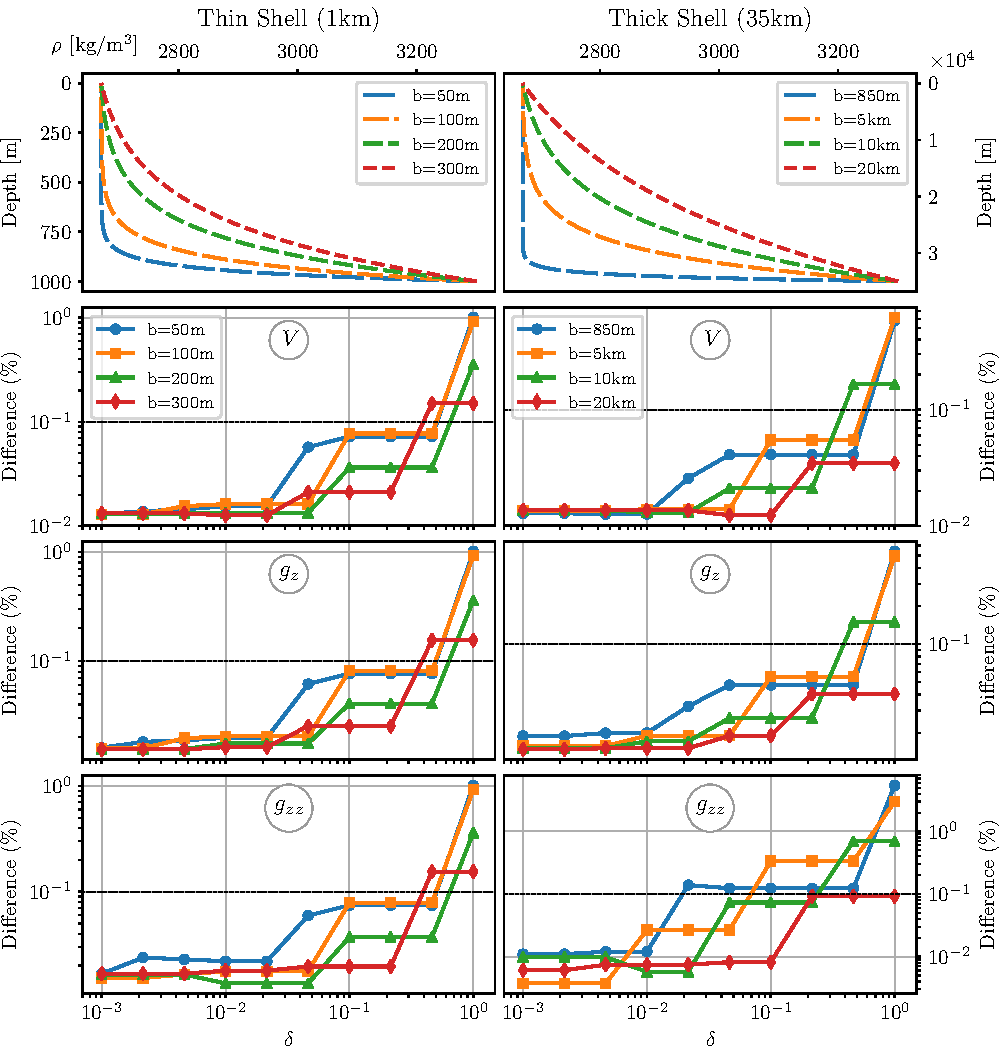
\includegraphics[width=\linewidth]{figures/exponential-delta.pdf}
\caption{
    Density functions used in the $\delta$ ratio determination and the 
    differences between the gravitational fields generated by the 
    numerical model and the analytical solution for a thin and a thick 
    spherical shell of 1km adn 35km of thickness, respectively, both 
    with the exponential density defined on equation 
    \ref{eq:density-exp}.
    A few values of the constant $b$ were used in order to test the 
    numerical model for different density variations.
    The computations were performed on the big grid described in 
    Table \ref{tab:grids}, with fixed values of the distance-size ratio 
    $D$ obtained for in the linear density case ($D=1, 2, 8$ for the 
    potential, gradient components and tensor components, respectively)
    and different values of the $\delta$ ratio.
    If the difference is less than 0.1\%, we consider that the model 
    has achieved an acceptable accuracy for the corresponding value of 
    $\delta$.
    }
\label{fig:delta-exponential}
\end{figure*}


%%%%%%%%%%%%%%%%%%%%%%%%%%%%%%%%%%%%%%%%%%%%%%%%%%%%%%%%%%%%%%%%%%%%%%%%%%%%%%%

\section{Implementation}

In order to perform the determinations of the distance-size and the 
delta ratio, we have developed a Python code that implements the 
discretization algorithms and the GLQ to finally compute the 
gravitational fields.

It is based on the pre-existing code developed by \citet{Uieda2016} (and 
included in Fatiando a Terra v.0.5, \citet{Uieda2013}) that computes 
the gravitational effects of tesseroids with homogeneous density.
Our implementation keeps the the homogeneous tesseroid calculation and 
the modified adaptive discretization algorithm while incorporates the 
new variable density computations with the density-based discretization 
algorithm.
On their software, \citet{Uieda2016} have optimised the more time 
consuming functions through the Numba compiler.
In contrast, we have decided to develop our new library in Cython 
language due to difficulties when passing a Python function as argument 
to precompiled Numba methods.

This new code is freely available under the BSD 3-clause open-source 
license and makes use of the pre-existing classes and functions of 
Fatiando a Terra v0.5 in order to define single tesseroid or meshes of 
them.
It can be downloaded from ...
\todo[inline]{include repo url}

\todo[inline]{I'm thinking to remove the speed comparison}

\subsection{Speed Comparison}

We have recorded the computation times for the gravity potential, the gradient component $g_z$ and the Marussi tensor component $g_{zz}$ generated by a single tesseroid model ($35$km of thickness) with homogeneous, linear and exponential density (with $b=50$km) at different heights. Then we calculated the ratio between these computation times:

\begin{equation}
    \text{Computation Times Ratio} =
        \frac{\Delta t_\text{variable}}{\Delta t_\text{homogeneous}},
    \label{eq:computation-times-ratio}
\end{equation}

\noindent where $\Delta t_\text{homogeneous}$ and $\Delta t_\text{variable}$ are the computation times corresponding to the homogeneous model and to the variable density ones (linear and exponential).

On Figures \ref{fig:speed-comparison}a and \ref{fig:speed-comparison}b we can see the results of these comparison.
In the linear density case the density-based discretization algorithm is not applied because the inequation \ref{eq:delta-density} is never satisfied.
For this reason, the homogeneous density model is up to 5 times faster than the variable density one in this case.
On the other hand, the density-based discretization algorithm makes the computation slower: up to 20 times slower than the homogeneous density code.
Nevertheless, this increase in the computation time pays off with a guarantee\todo[inline]{guarantee is a noun?} on its accuracy.

\begin{figure}
\centering
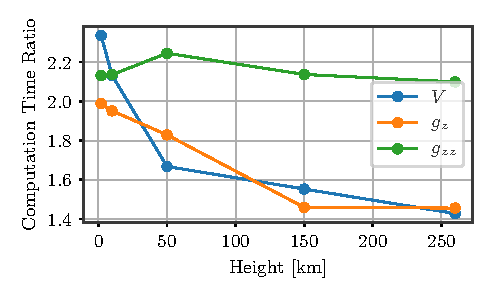
\includegraphics[width=0.9\linewidth]{figures/speed-comparison.pdf}
\caption{Computation time ratio between a single tesseroid model with variable and with homogeneous density at different heights (defined in equation \ref{eq:computation-times-ratio}) for (a) a linear and (b) an exponential density.}
\label{fig:speed-comparison}
\end{figure}


%%%%%%%%%%%%%%%%%%%%%%%%%%%%%%%%%%%%%%%%%%%%%%%%%%%%%%%%%%%%%%%%%%%%%%%%%%%%%%%

\section{Example with real data}

Besides the determination of the distance-size and the delta ratio, we 
wanted to illustrate how the algorithm performs under a real data model.
For this task we have chosen the Neuqu\'en Basin: a sedimentary basin 
located to the east of the Andes, between 32$^\circ$S and 40$^\circ$S latitude 
(see Figure \ref{fig:neuquen-basin}a), that includes continental and marine 
siliciclastics, carbonates and evaporites accumulated over the Jurassic and 
the Cretaceous constituting a stratigraphic record up to 5000m of depth 
\citep{Howell2005}.

\begin{figure*}
\centering
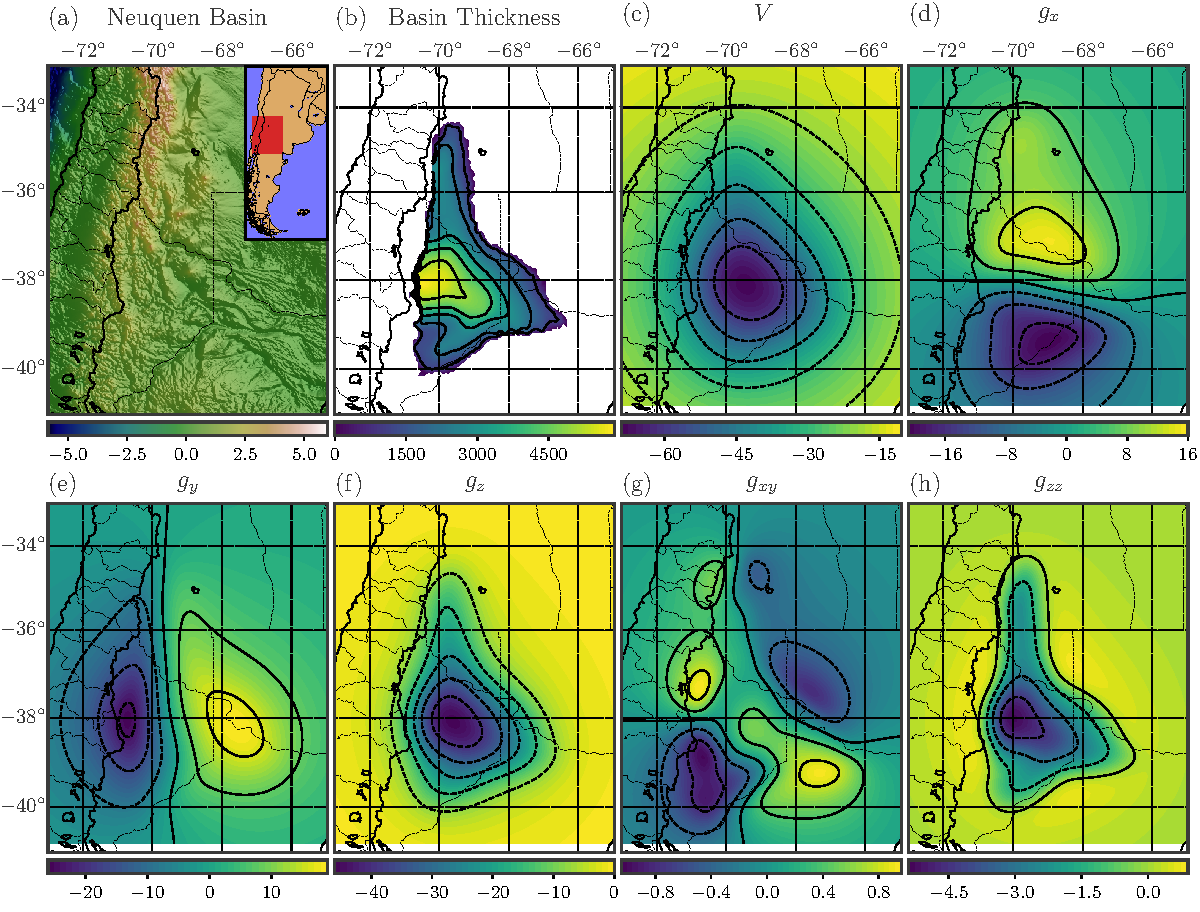
\includegraphics[width=\linewidth]{figures/neuquen-basin.pdf}
\caption{
    Forward model example with real data: Nequ\'en sedimentary modelled 
    through tesseroids with exponential density.
    (a) Topography of Neuqu\'en Basin (in km),
    (b) thickness of the sedimentary basin (in meters),
    (c) density function used to model the basin (depth in km and density in 
    kg/m$^3$),
    (d)-(l) computed gravity fields: potential $V$ (in J/kg), gradient 
    components $g_x$, $g_y$ and $g_z$ (in mGal) and Marussi tensor components 
    (in Eötvös), calculated at 50km of height over the ellipsoid.}
\label{fig:neuquen-basin}
\end{figure*}

The thickness of the sediment pack was obtained from \citet{Heine2007}.
We managed to produce a regular grid with a resolution of 0.05$^\circ$ on both 
longitude and latitude directions with one value of thickness on each node 
(see Figure \ref{fig:neuquen-basin}(b)).

In order to compute the gravity fields generated by this basin we created a 
mesh of tesseroids, each one located on one of the nodes of the grid, with 
dimensions of 0.05$^\circ$ $\times$ 0.05$^\circ$ and depth equal to the 
thickness of the basin on the corresponding node.

We must also define a density function for the entire model. 
\citet{Sigismondi2012} measured a minimum and maximum density contrast for 
the Neuqu\'en basin of -412kg/m$^3$ and -275kg/m$^3$, respectively.
So we have chosen, for this specific example, an exponential density (like the 
one in equation \ref{eq:density-exp}) that assumes the minimum value on the 
surface and the maximum at 5858m, i.e. the bottom of the basin, with a value 
of $b$ equal to 2km.
This density function can be seen on Figure \ref{fig:neuquen-basin}(c).

We have computed the gravity potential $V$, the gradient components $g_x$, 
$g_y$ and $g_z$, and the Marussi tensor components $g_{xx}$, $g_{xy}$, 
$g_{xz}$, $g_{yy}$  and $g_{zz}$ on a computation grid of 159$\times$163 nodes 
with a 0.05$^\circ$ spacing on both longitude and latitude directions at a 
50km height over the reference ellipsoid.
The resulting gravity fields can be seen in Figures 
\ref{fig:neuquen-basin}(d)-(l).
We have excluded the other components of the Marussi tensor from the Figure, 
although they can be found in the repository.


%%%%%%%%%%%%%%%%%%%%%%%%%%%%%%%%%%%%%%%%%%%%%%%%%%%%%%%%%%%%%%%%%%%%%%%%%%%%%%%

\section{Conclusions}

We have developed a new methodology that computes the gravitational fields 
generated by a tesseroid with continuously variable density in depth.
It numerically solves the integrals that define the gravitational potential, 
its gradient and the Marussi tensor components through the Gauss-Legendre 
Quadrature (GLQ), which essentially consists in approximating the 
gravitational fields of the tesseroids with the effect of point masses located 
on nodes of the Quadrature.

Instead of enhancing the accuracy of the method by increasing the order of the 
GLQ on each integration, we make use of the pre-existing modified adaptive 
discretization algorithm and a new density-based discretization algorithm.

The former one divides the tesseroid by half if the ratio of the distance to 
the computation point and its size is lower than a predefined distance-size 
ratio $D$.
This algorithm is introduced in order to minimise the error when the 
computation point is close to the tesseroid, in which case the effect of the 
point masses becomes more noticeable and the approximation lose precision.
Following this idea, we can summarise that the distance-size ratio $D$ 
controls the accuracy of the method: a higher value of $D$ generates more 
divisions of the tesseroids, thus more point masses, what leads to a more 
precise approximation.
Nevertheless, this algorithm is not sufficient to guarantee the accuracy of 
the method in case of tesseroid with variable density.

For this reason we have developed a density-based discretization algorithm that 
divides the tesseroid on the radius at which the \emph{maximum variation} of 
the density function takes place, only if a certain inequation that relates 
this \emph{maximum variation} with a predefined delta ratio $\delta$ holds.
The number of subdivisions is indirectly controlled by this delta 
ratio $\delta$, and thus the accuracy of the computation.
This new algorithm is intended to minimise the error due to the inability of 
the GLQ to produce precise approximations in case of highly varying density: 
the information about the density function is summed up with the values that 
it assumes at the node of the quadrature.
Increasing the subdivisions of the tesseroid where the \emph{maximum 
variation} of the density takes place becomes an efficient way to reduce this 
kind of error.

Because there is no direct relation between the values assigned to $D$ and 
$\delta$ with the error of the computation, we had to empirically determine 
the minimum value of $D$ and the maximum value of $\delta$ that produce an 
acceptable accuracy for each gravitational field, while maintaining an 
efficient computation.
The default values of $D$ and $\delta$ must produce accurate computations for 
most continuous and smooth densities, that's why we have chosen two density 
functions in order to establish them: a linear and an exponential one.

In the linear density case, the densty-based discretization algorithm is not 
applied due to how it's build, so only a default value of $D$ had to be 
determined.
By comparing the analytical solutions of the gravitational fields generated by 
a spherical shell with the ones produced by the numerical model for different 
values of $D$, we have obtained default values for the distance-size ratio of 
1, 2 and 8 for the potential, its gradient and the Marussi tensor components, 
respectively.
From these comparisons we can guarantee a precision of 0.1\% or greater on the 
computations of the gravitational fields generated by any tesseroid with a 
linear density.

The exponential density case is more complex, due to the fact that both $D$ 
and $\delta$ must be determined simultaneously.
We have explored regular gridded points in the $D$, $\delta$ space and 
computed the percentage difference between the analytical solutions for a 
spherical shell and the numerical model.
We had to take into account that the $D$ values cannot be lower than the ones 
determined for the linear density case due to the fact that they must 
guarantee acceptable accuracy for every continuous density function, including 
the linear one.
From these comparisons we have concluded that the more efficient computations 
take places when the $D$ values obtained in the linear density scenario are 
used, i.e. the minimum ones.
This can be understood in terms of which kind of discretization produces more 
subdivisions: a higher $D$ may produce more discretizations than a lower 
$\delta$ because the first one divides the tesseroid in the radial, longitude 
and latitude directions, while the latter only divides it in the radial 
direction.
In conclusion, we found out that keeping the $D$ values as the ones obtained 
for the linear density case, a $\delta = 0.2$ is needed for the computation of 
the potential and its gradient components, while a $\delta = 0.01$ must be 
used for the Marussi tensor components in order to ensure a 0.1\% precision.

In order to implement this new methodology we have developed a Python code 
that carries out both discretization algorithms and the gravitational field 
computation through the GLQ. It's freely available under the BSD 3-clause 
open-source license and can be downloaded from
\todo[inline]{add repo url}

Finally, we have shown how this new method performs under a real data example: 
we have computed the gravitational fields generated by the Neuqu\'en 
sedimentary basin through a tesseroid model with an increasing exponential 
density in depth on a regular grid at a computation height of 50km over the 
reference ellipsoid.


%%%%%%%%%%%%%%%%%%%%%%%%%%%%%%%%%%%%%%%%%%%%%%%%%%%%%%%%%%%%%%%%%%%%%%%%%%%%%%%

\section{Acknowledgments}

We are indebted to the developers and maintainers of the open-source
software without which this work would not have been possible.

%%%%%%%%%%%%%%%%%%%%%%%%%%%%%%%%%%%%%%%%%%%%%%%%%%%%%%%%%%%%%%%%%%%%%%%%%%%%%%%

\bibliographystyle{gji}
\bibliography{references}

\end{document}
